The following section describes the simulated base case, with a focus on the key performance indicator (KPI). The KPI represents the material recycling rate, and measures the percentage of household waste, which is recycled. The "base case" simulation does not include any extra efforts from Oslo municipality to influence waste sorting behavior. Note that the simulation only considers food, plastic, rest waste, and paper/cardboard, while glass/metal, textiles and garden waste is excluded. It also only represents the target group, not the whole population in Oslo.  

\indent \newline
Sections later in the chapter presents five recommended initiatives for Oslo municipality to improve the material recycling rate. The effects and outcomes of the practical initiatives will be analyzed and ranked, based on which initiative will have the most effect on waste sorting behavior and the material recycling rate.  

\section{Base Case}

\indent \newline
The "base case" represents a situation without any initiatives from Oslo municipality on waste sorting behavior. The result shows a small increase in the material recycling percentage. As shown in figure 5.1, the material recycling rate increases slightly and reaches 31.69\% by 2030. The graph represents the current state of Oslo's material recycling rate, which will not increase further without extra efforts or initiatives from Oslo municipality. The variable "material recycle percentage" is influenced by how many tons of waste that are collected of each "category", and waste sorting behavior. It is imperative to influence waste sorting behavior in order for the material recycling percentage to increase further. 

\begin{figure}[H]
\centering
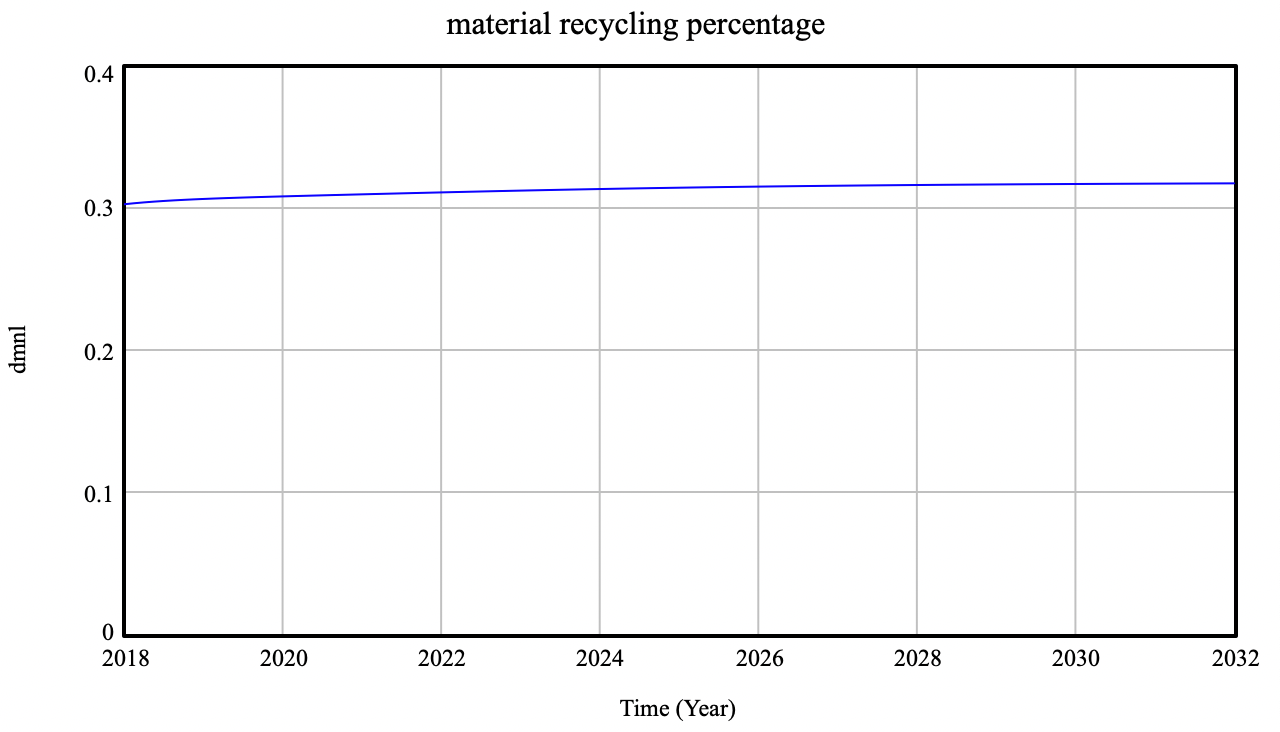
\includegraphics [scale=0.28,angle=360]{figures/basecase.png}
\caption{Base Case}
\label{fig:basecase}
\end{figure}

\indent \newline
The figure above shows that the graph (material recycling percentage) has a steeper increase during the first couple of years, while the graph stagnates when it gets closer to year 2030. This is due to the rate of change in waste sorting behavior. 

\indent \newline
An analyze of figure 5.2 below, demonstrates that the change in waste sorting behavior starts at an elevated level and decreases over time. With comparison to material recycling percentage, the graph stagnates as it moves towards 2030. Waste sorting behavior in practice is determined through the changes in waste sorting behavior. According to the graph, waste sorting behavior in practice has a greater increase during the first couple of years, while it levels out when getting closer to 2030. This is because the target group is adjusting their waste sorting behavior over time. This represents the early adopters of the target group. 

\begin{figure}[H]
\centering
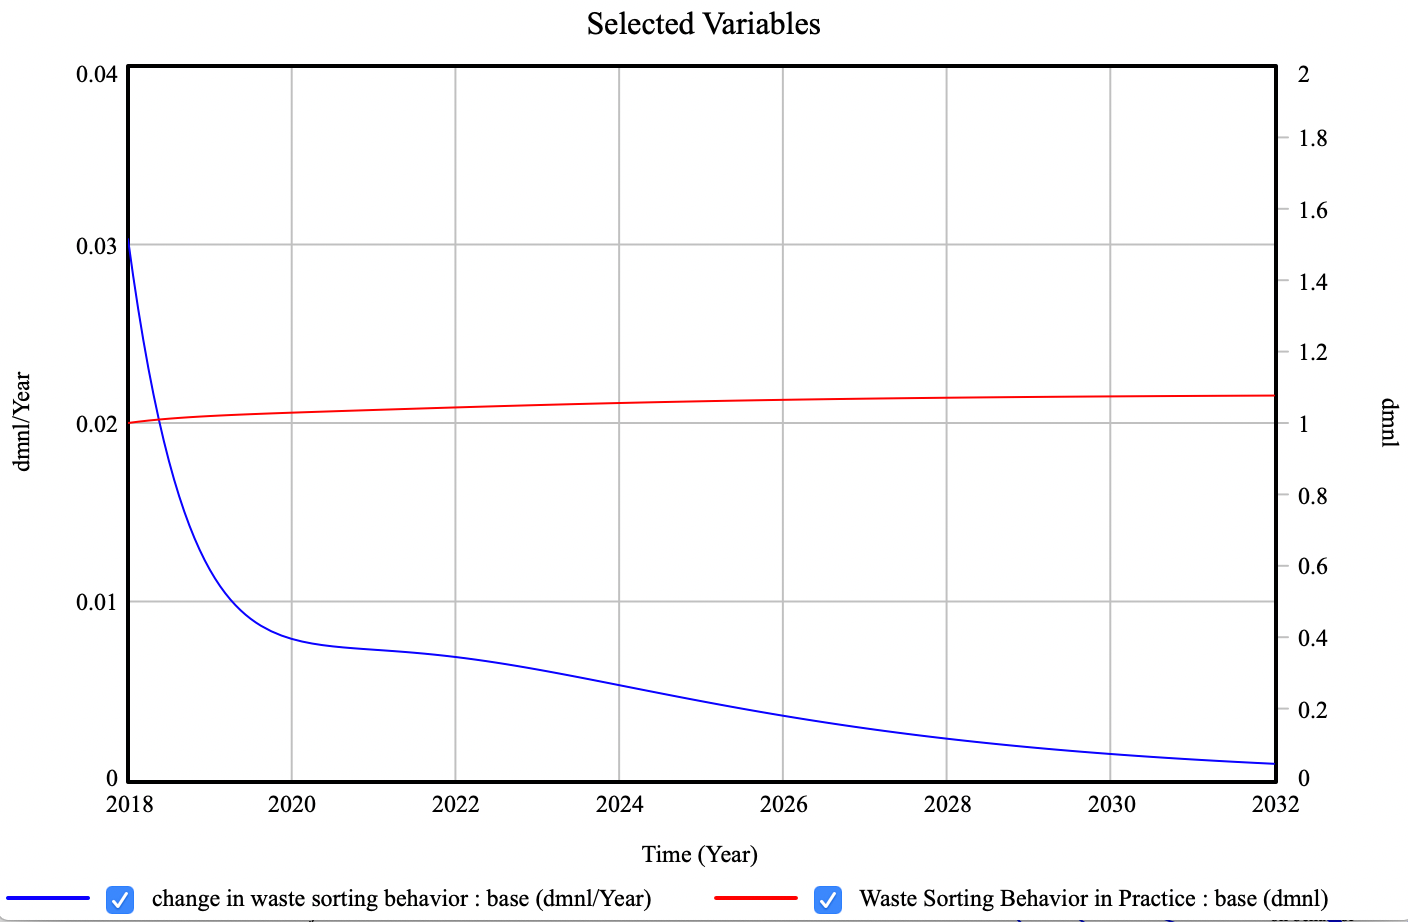
\includegraphics [scale=0.28,angle=360]{figures/basecase2.png}
\caption{Waste Sorting Behavior}
\label{fig:basecase2}
\end{figure}

\indent \newline
The results from the base case simulation indicates that Oslo municipality will not be able to reach the desired recycling rate by 2030. The next part of the chapter describes how the municipality, through additional efforts and initiatives, can improve the recycling percentage in order for them to reach their main goal. 

\section{Initiatives}

\indent \newline
The simulated model is based on five different initiatives Oslo municipality can make use of to improve the recycling percentage. Each of the scenarios is simulated separately to show an isolated effect of the initiatives.

\subsection{Increase Advertising Effectiveness}

\indent \newline
The first initiative consists of increasing advertising effectiveness. It is essential that Oslo municipally increases their marketing spend towards people aged 20-39. Currently, the marketing effect is too low and more effective marketing campaigns in the appropriate channels is needed. Research suggests that the target group needs more information about what the waste goes to after the garbage is thrown \cite[p. 72]{recycling}. The main focus of the marketing will therefore be on explaining the benefits and values of sorting the waste in the right waste container, and the effect of each contribution. 

\indent \newline
In order to reach out to the target group, the municipality should use Snapchat, Facebook, Linkedin, Twitter and Instagram as marketing channels to communicate with the audience. It is also recommended that the communication through these channels consist of the benefits and importance of  recycling waste in the right containers placed in the condominiums. 
The initiative is realistic to implement. Oslo municipality is already doing some advertising at the moment, mostly through television advertisements and Instagram. An assumption is that they already have an advertising department who can start the suggested advertising process, without investing too much in personnel and resources. 

\indent \newline
The target group needs additional information to change their waste sorting behavior. Therefore, a reliable source of information and communication is critical. It is Oslo municipality's responsibility to provide understandable and clear information through these channels. They would answer questions like what and how to sort specific waste. 

\begin{figure}[H]
\centering
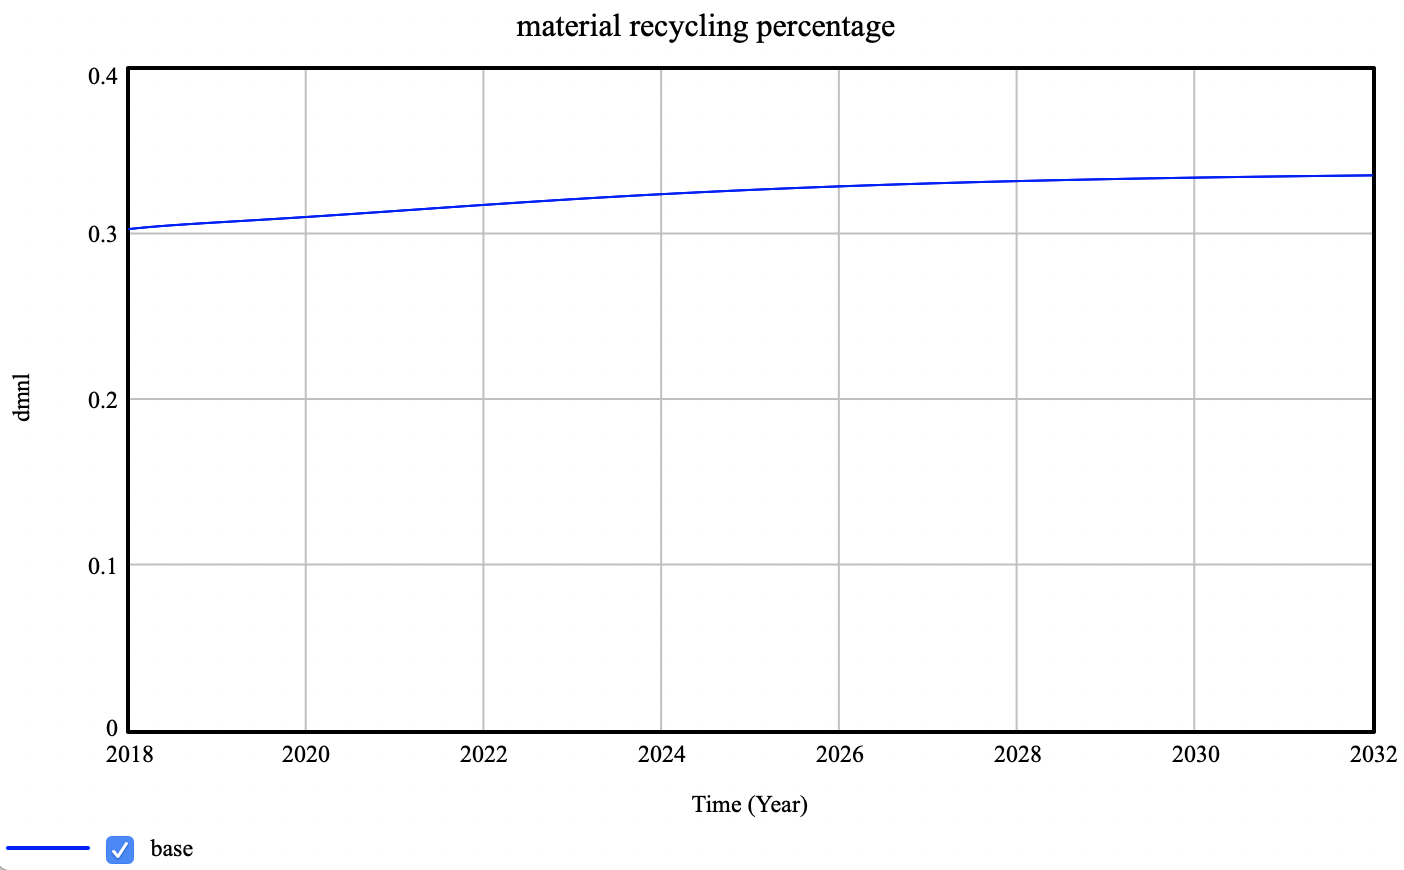
\includegraphics [scale=0.28,angle=360]{figures/advertisingeff.png}
\caption{Increasing Advertising Effectiveness}
\label{fig:advertisingeff}
\end{figure}

\indent \newline
In the figure above, the blue line represents the material recycling percentage and the effect is displayed in the time interval 2018-2030. The graph visualizes an isolated effect of marketing on the recycle percentage, which leads to a final recycling percentage of 33.38\%. Compared to the base case this is an increase of 1.69 percentage points, given that the other variables included in the base case do not affect  the recycling rate. The result shows the effect of marketing in the first 7 years and then the growth declines. This reflects that the majority of the market has been reached, which leads to a lower adoption rate. Improvements of the recycling percentage is related to the stock "advertising effectiveness in practice" and the desired goal is to adjust household knowledge and attitude towards waste sorting. As expected, the results indicate a realistic increase in behavior of the target group which affects the recycling percentage. 

\subsection{New Quality of Collected Waste}

\indent \newline
The following initiative represents a situation where there are three waste containers per apartment complex, one for plastic, paper and rest waste. In this scenario, Oslo municipality has to increase the number of waste containers in order to improve the quality of the collected waste. Increasing the quality of collected waste also increases the material recycling percentage, and reduces the amount of residual waste. The main objective in this initiative is providing even better material recycling options. That way, the population can recycle the material in more detail from their homes. This will result in less efforts from Oslo regarding material recycling. 

\begin{figure}[H]
\centering
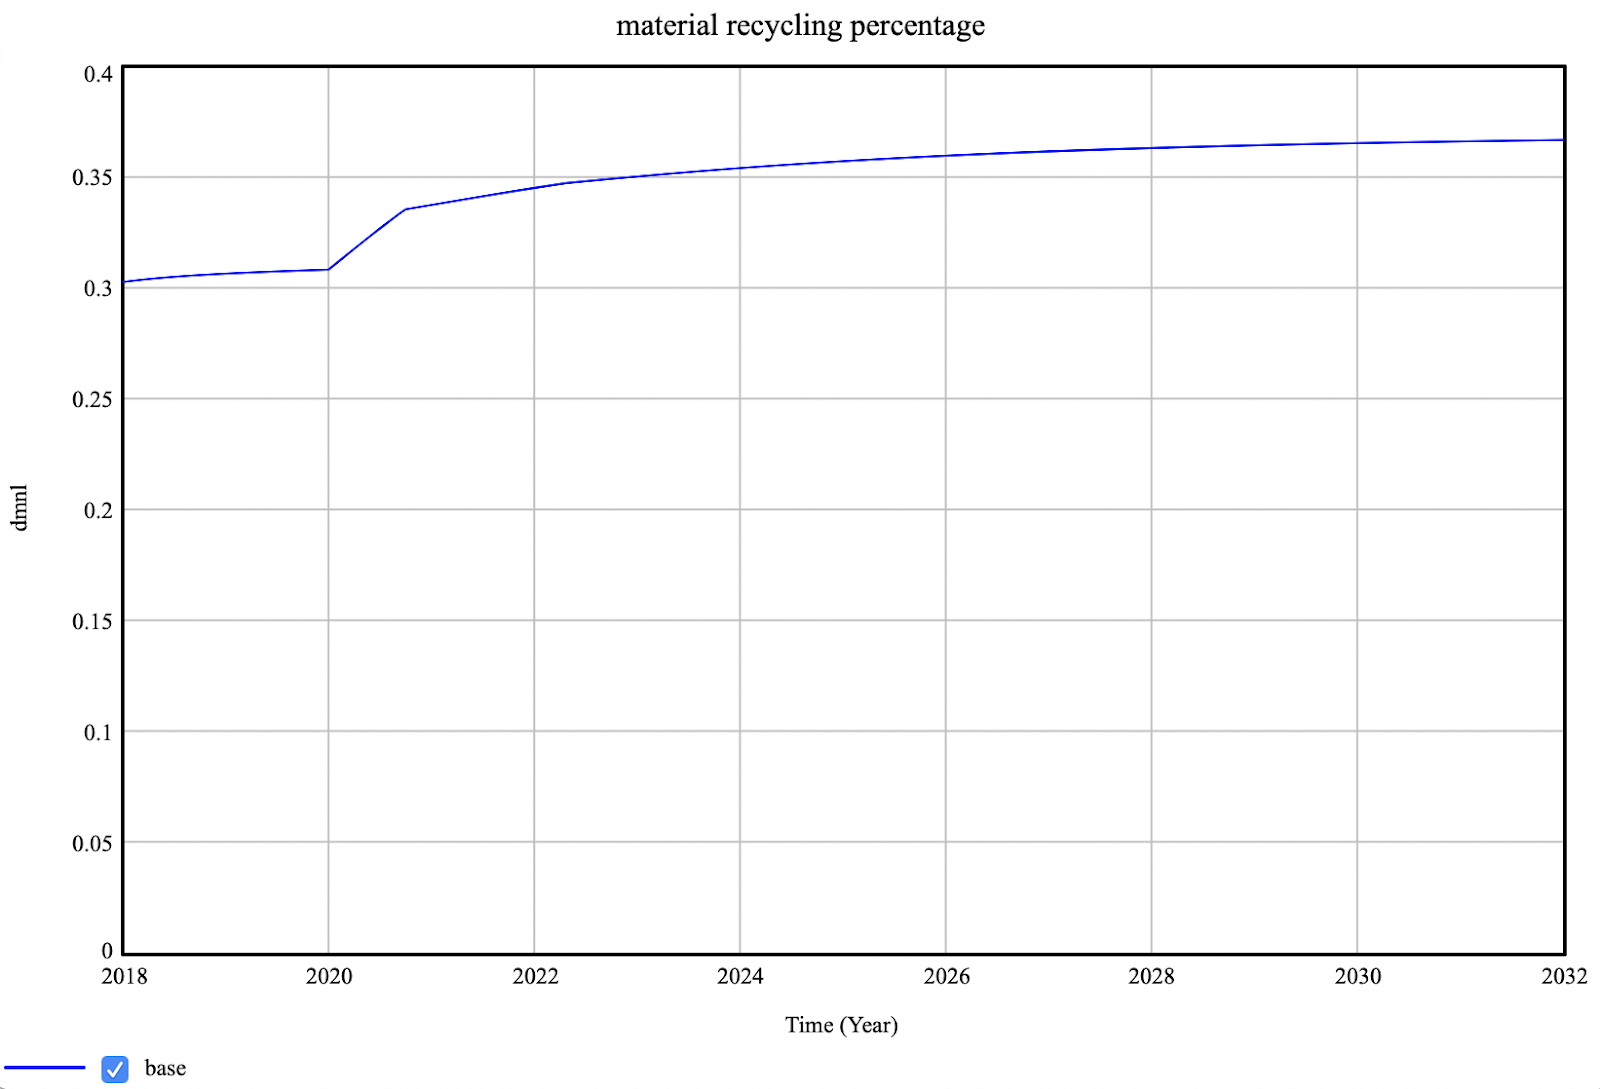
\includegraphics [scale=0.24,angle=360]{figures/newquality.png}
\caption{New Quality of Collected Waste}
\label{fig:newquality}
\end{figure}

\indent \newline
The graph in figure 5.4 represents an isolated effect of an increase of  "quality of collected waste", in other words, the installation of new waste containers. There is a greater increase in the first year, where Oslo municipality introduces new waste containers. After the introduction year, the growth stabilizes due to citizens adapting to the new sorting system. Through implementation of new containers, the recycling percentage increases from 31.69\% in the base case to an improved material recycling percentage of 36.53\%. This results in an increase of 4.84 percentage points and the greatest impact of the initiatives on the model. The implementation of the new containers is represented through the variable "new quality of collected waste", where the initial value is increased from 1 to 2. This means the quality of the sorted waste will increase with 100\%, which might seem like a lot, but it is plausible to assume that more waste containers will have a significant impact on this stock. 

\subsection{Improvements in Waste Management System}

\indent \newline
The third initiative is to implement and utilize smart waste containers for Oslo's apartment buildings. This will ultimately help optimize the frequency of waste collection and the volume of waste containers in the long term. The main concept of the smart containers is that they will automatically compress the waste in the containers. An additional feature is to implement a measuring devices in the waste containers, which will intelligently measure the amount of waste in the containers. The sensors within the containers collect data, which is sent to a server for evaluation and analysis. The results of measurements are displayed in a web platform for the consumers and the waste collection firm to see \cite{smart}

\indent \newline
An additional feature would be to develop an application for smart devices (smart phones, PC, and tablets), where the consumer and collection firm can monitor the current status of the specific waste containers. The consumer will get notified if the container is full, while the waste management company will know when to collect the waste. This data can easily be analyzed, which will help the waste management company to forecast when the container is full, allowing them to plan future routes. The addition of the smart application will increase cost-efficiency and improve the target group's waste sorting behavior. Ultimately, the waste container mechanisms should be driven by solar panel technology, which will help to sustain the system in the long term. 

\begin{figure}[H]
\centering
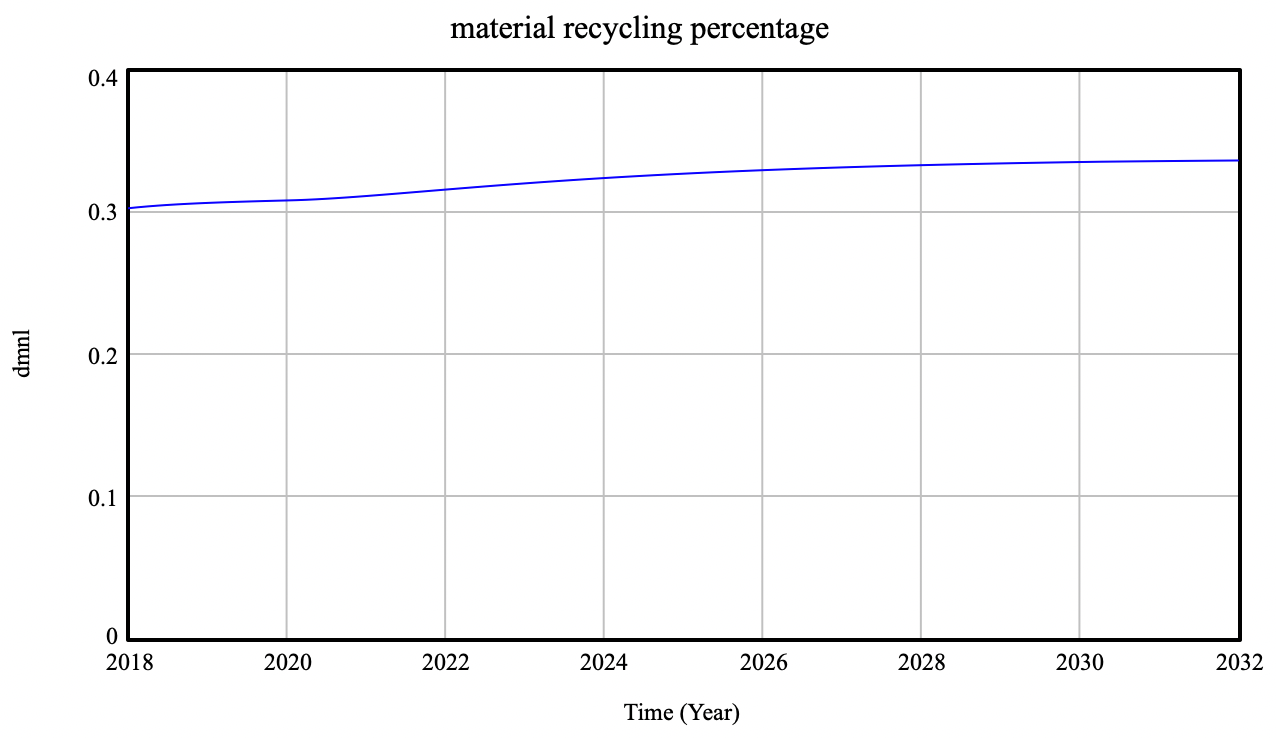
\includegraphics [scale=0.28,angle=360]{figures/improvementsinitiative.png}
\caption{Improvements in Waste Management System}
\label{fig:improvementsinitiative}
\end{figure}

\indent \newline
The simulation results of implementation and utilization of smart containers is displayed in the figure above. Compared to the base case, the effect of smart containers on material recycling percentage is quite positive. An implementation of this initiative leads to an increase in the material recycling rate from the original 31.69\% to 33.86\%. This represents an increase of 2.17 percentage points. The effect of smart containers is implemented in the simulation model through the variable "investments in new waste management system", and increases the value from 1 to 2, which seems to be a realistic value. The implementation of smart containers also positively affects the exogenous variables "new volume of containers" and "new frequency of waste collection". As mentioned earlier, the collection firm can now plan future routes and optimize the frequency of waste collection. They can also simulate patterns for each apartment building and adjust the volume of containers based on the results. The volume is also affected when the containers have the ability to compress the containing waste. 

\indent \newline
The initiative appears to be realistic since the technology already has been developed and being implemented in e.g. Trondheim municipality. There are however implementation costs related to this initiative, but the profit will most likely exceed the costs through optimizing frequency of waste collection and the volume of containers in the long term. 

\subsection{Economic Incentives}

\indent \newline
The fourth initiative is to implement economic incentives to improve the attitude towards waste sorting. According to research, the designated target group would perform better if Oslo municipality provided economic incentives to the residents of apartment complexes \cite[p. 46]{Mikkelborg}. However, it is quite challenging to measure individual waste sorting behavior, as there is no realistic method or system of measuring this. An alternative is to offer a shared economic incentive, based on a given apartment complex. 

\indent \newline
A suggestion is to cut a portion of the shared costs that are related to Oslo municipality's fees and taxes. This will be based on the quality of sorted waste with regards to the apartment building. Furthermore, this would create a culture around waste sorting behavior, and strengthen the community to collaborate to reach the level where economic incentives are generated. This initiative would affect several variables in the long term. Variables such as social pressure, mirroring behavior and intention action gap would either increase or decrease.

\begin{figure}[H]
\centering
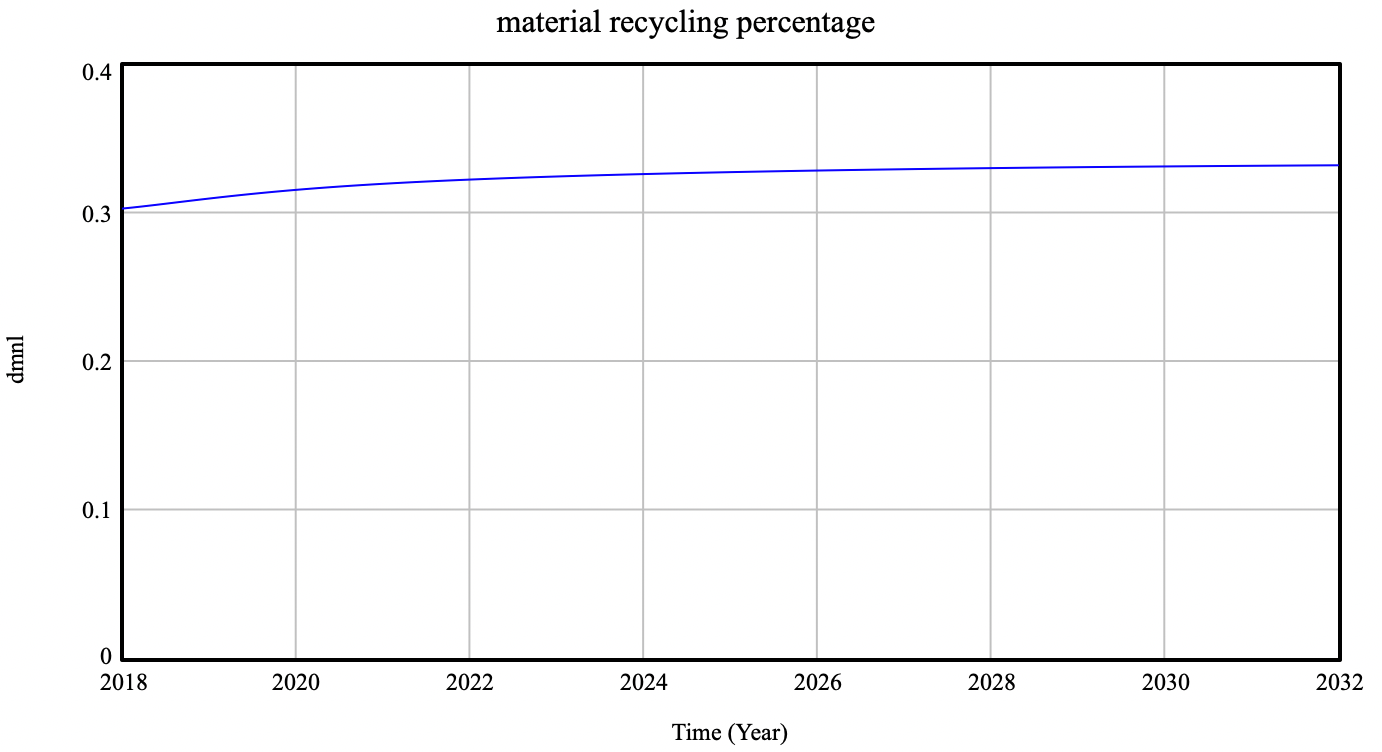
\includegraphics [scale=0.28,angle=360]{figures/incentives.png}
\caption{Economic Incentives}
\label{fig:incentives}
\end{figure}

\indent \newline
In the graph above (figure 5.6), the isolated effect with regards to the implementation of monetary benefits is displayed. Compared to the base case, the material recycle percentage increases from 31.69\% to 33.11\%, which is an increase of 1.42 percentage points. To implement the initiative in the simulation model, the exogenous variable "monetary benefits" is adjusted from 1 to 3. This is a realistic increase, since the target group's motivation will be influenced by monetary benefits. This will also increase the attitude towards waste sorting almost instantly. The implementation of this initiative is both realistic and practical. If Oslo municipality is willing to invest in this initiative, it wouldn't be too challenging to implement. 

\subsection{Increase Frequency of Waste Collection}


\indent \newline
The fifth and final initiative is to increase the frequency of waste collection. Increasing the frequency of waste collection will potentially have a positive influence on waste sorting behavior. There are instances where certain containers get full before the waste collection occurs. This results in garbage bags going in the wrong waste container or being placed on the side/street. Optimizing the waste collection frequency will prevent the waste containers from getting overloaded, and thus improving waste sorting behavior.  

\begin{figure}[H]
\centering
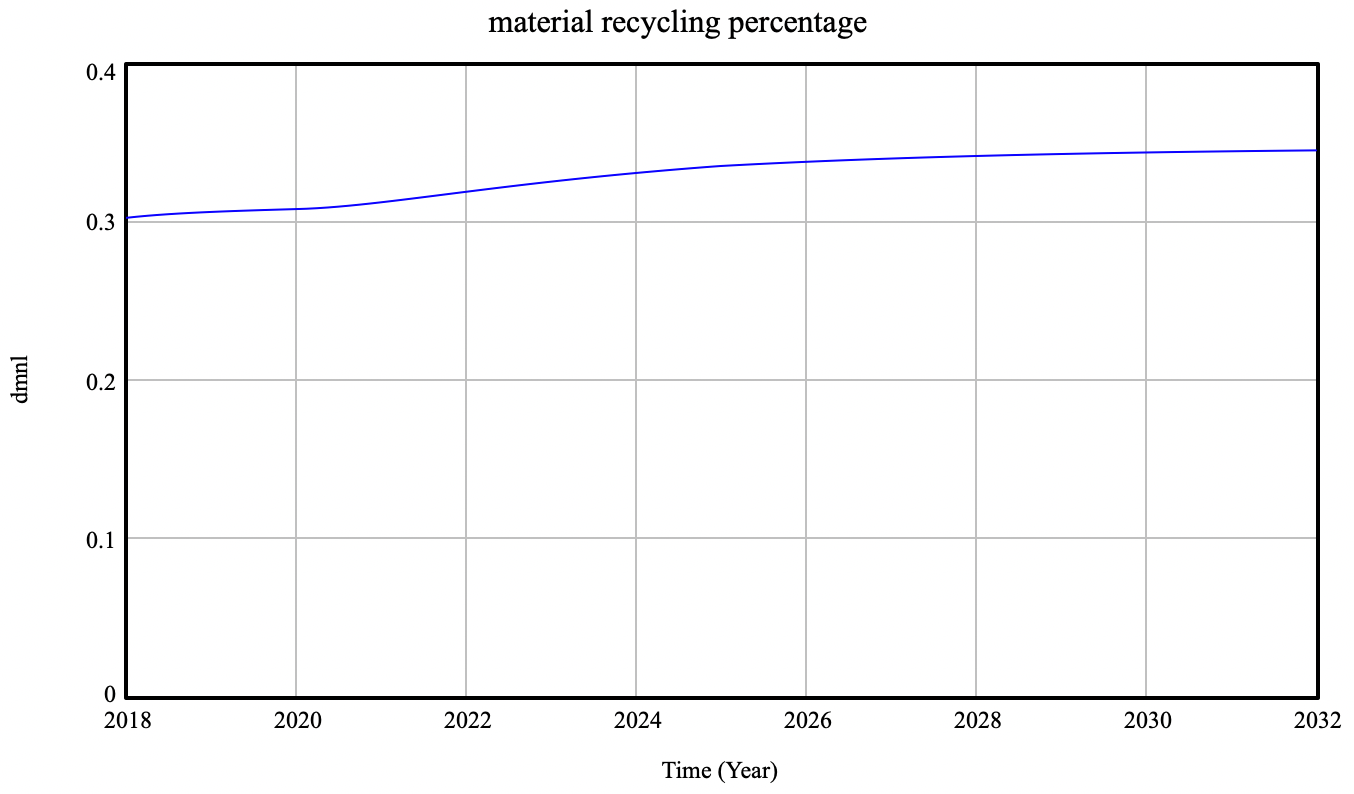
\includegraphics [scale=0.28,angle=360]{figures/frequencyinitiative.png}
\caption{Increasing Frequency of Waste Collection}
\label{fig:frequencyinitiative}
\end{figure}

\indent \newline
The graph in figure 5.7 represents the isolated impact of changing the frequency of waste collection. The material recycling percentage increases from the original 31.69\% to 34.4\%. The total increase in this initiative is 2.71 percentage points. The graph starts out relatively stable and acquires a greater increase after 2020. The reason for this is the variable "introduction year of new frequency". The graph stagnates as it gets closer to 2030 because, by that time, the initiative will have reached its maximum potential. The recommended initiative seems realistic because the implementation of this concept is pretty straight forward, and results in a direct effect on waste sorting behavior. 

\section{Rankings \& Recommendations}

\indent \newline
The figure and table below compares the different initiatives in terms of their effect on the material recycling percentage. The reasoning behind this is to rank the initiatives in order to give the best recommendations to Oslo municipality when it comes to improving the material recycling percentage. 

\begin{figure}[H]
\centering
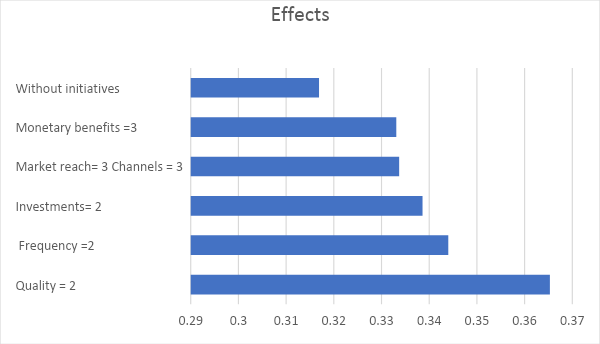
\includegraphics [scale=0.50,angle=360]{figures/rankedinitiatives.png}
\caption{Initiative Scores}
\label{fig:rankedinitiatives}
\end{figure}

\begin{table}[H]
\centering
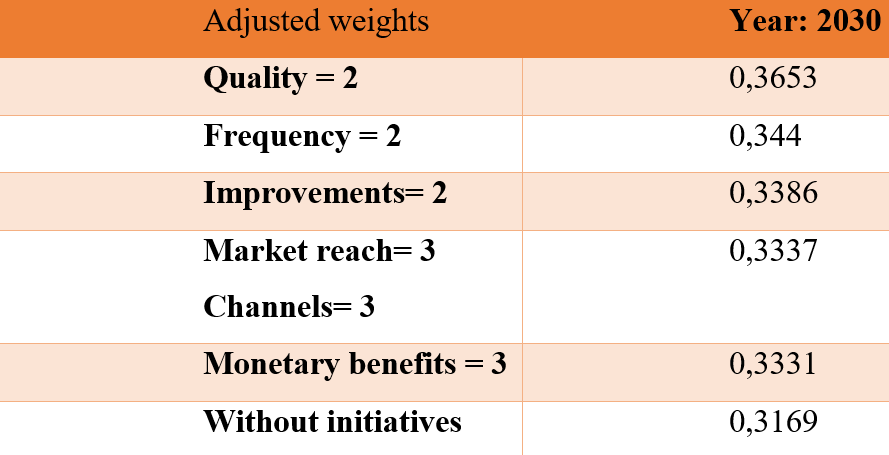
\includegraphics [scale=0.28,angle=360]{tables/rankedinitiatives.png}
\caption{Ranked Initiatives}
\label{tbl:rrankedinitiatives}
\end{table}

\indent \newline
When these five initiatives are separated and simulated individually, there is a similar change in the material recycling percentage. The graphs often have a comparable shape and increases in the interval between 2 and 4 percentage points. Certain initiatives are easier to implement, and therefore takes less time for the effects to kick in. This may, however, result in a reduced impact.

\indent \newline
According to the table above, improving the quality of collected waste is the initiative with the highest impact on the material recycling rate, with a rate of 36.53\%. The second-best initiative is improving the frequency of waste collection, with a rate of 34.4\%. The common denominator between these two initiatives is that they are moderately easy to implement in the real world. It does not require a lot from either Oslo municipality or the consumers. The last of the top 3 initiatives is investing in a new waste management system. This initiative is tougher to implement and execute because it requires more effort and funding from Oslo municipality. The initiative is sustainable in the long term and doesn't require extra efforts from the consumers. It makes life easier for both the collection firm and the target group, with a strong potential for optimizing collection routes. 

\indent \newline
To increase the probability of reaching a 50\% recycling rate by 2030, Oslo municipality should implement these initiatives. Since this paper only focuses on a part of the total population in Oslo, a 50\% recycling rate will be difficult to achieve based on the simulation model. However, these initiatives are still alternatives which will improve the current situation.

\indent \newline
The following part of the paper presents a sensitivity analysis to test the different initiatives in various scenarios.  

